\chapter{Methodology}

To gain insights into the proposed methods for researching the appliance of (ND)-Laplace for cluster algorithms we conducted experiments.
The experiment results are used to evaluate our method against other literature.
In this chapter we explain:
\begin{enumerate}

  \item Datasets
  \item Environmental setup.
  \item For each research question: Description of the different experiments.
  \item For each research question: Results.
\end{enumerate}

\section{Datasets}
For this research, we will use a synthetic dataset for all three research questions.
In addition to this, we used the LSun dataset as a lot of comparable literature uses this as well for evaluation.
\todo[inline]{Describe LSun dataset}
% Please add the following required packages to your document preamble:
% \usepackage{booktabs}
\begin{table}[h]
  \begin{tabular}{@{}lllll@{}}
    \toprule
    Records & Centers & Dimensions & Standard deviation & Research \\ \midrule
    50      & 4       & 2          & 0.60               & RQ 1     \\ \bottomrule
    50      & 4       & 3          & 0.60               & RQ 2     \\ \bottomrule
    50      & 4       & 5          & 0.60               & RQ 2     \\ \bottomrule
  \end{tabular}
\end{table}

Research question 3 uses a "real-world" dataset to properly assess the different dataset properties that are the subject of this research question.
\todo[inline]{Describe datasets (RQ3)}
\section{Environmental setup}
For running the experiments we make use of 16GB ram memory and i7-10750H 2.6Ghz processor.
The experiments are run using a Docker container which runs a pre-configured distribution of Linux Alpine.
It includes a pre-installed Anaconda environment for python \footnote{https://github.com/devcontainers/images/tree/main/src/anaconda}\footnote{tag: mcr.microsoft.com/devcontainers/anaconda:0-3}.
We run the container using the dev-container feature for visual-studio code \footnote{https://code.visualstudio.com/docs/devcontainers/containers}.
This allows us to create a reproducible experiment environment.
\newpage
\subsection{Libraries \& code versions}
We use python version 3.9.13 with Jupyter notebook for creating a reproducible experimental environment.
The packages for python are:
\begin{enumerate}
  \item Scikit-learn: 1.0.*
  \item Yellow-brick: 1.5
  \item Numpy: 1.24.*
  \item Pandas: 1.4.*
  \item Seaborn: 0.11.*
  \item Mathplotlib: 3.5.*
\end{enumerate}

\section{Methods}
This section explains what methods/ algorithms we used and how we evaluate them.
\subsection{Clustering methods}
For the three different algorithms: K-Means, \gls{ap} and \gls{dbscan} we analyzed the most important decisions regarding parameter selection.
In this section, we give a short list and explanation of the different parameters we used throughout the experiments.
For all three Sklearn was used, and for each of them we also provide the underlying formula.
\subsubsection{K-Means}
\todo[inline]{Work in progress}
\begin{equation}
  \sum_{i=0}^{n}\min_{\mu_j \in C}(||x_i - \mu_j||^2)
\end{equation}
\begin{table}[h]
  \begin{tabular}{|c|c|c|}
    \hline
    Parameter & Description & Value \\
    \hline
  \end{tabular}
  \caption{K-Means provided by the Scikit-learn package}
  \label{tab:kmeans-formula-sklearn}
\end{table}
\subsubsection{Affinity Propagation}
\todo[inline]{Work in progress}
\begin{table}[h]
  \begin{tabular}{|c|c|c|}
    \hline
    Parameter    & Description  & Value        \\
    \hline
    Row 1 Data 1 & Row 1 Data 2 & Row 1 Data 3 \\
    \hline
  \end{tabular}
  \caption{Affinity Propagation provided by the Scikit-learn package}
  \label{tab:ap-formula-sklearn}
\end{table}
\subsubsection{DBSCAN}
\todo[inline]{Work in progress}
\begin{table}[h]
  \begin{tabular}{|c|c|c|}
    \hline
    Parameter    & Description  & Value        \\
    \hline
    Row 1 Data 1 & Row 1 Data 2 & Row 1 Data 3 \\
    \hline
  \end{tabular}
  \caption{DBSCAN provided by the Scikit-learn package}
  \label{tab:dbscan-formula-sklearn}
\end{table}

\subsection{Evaluation}
With differential privacy, it is a trade-off of utility versus privacy.
Therefore, for the evaluation of the 2D/3D-Laplace algorithms, we compare both criteria to achieve a consensus between utility and privacy.
\subsubsection{Utility}
Based on chapter \ref{theory:evaluate}, we can conclude that the corresponding literature mainly evaluates one clustering algorithm and not multiple ones.
Because of this, we do not use any internal validation; because the different types of metrics are too easily influenced by the choice of clustering algorithm.
Instead, we decided to pick up external validation methods similar to other studies as well.
They did use either Rand Index or Mutual Information, but because both have different strengths we evaluate both.

It is not likely that we will use many data points for research questions 1 and 2.
To compensate for this, the adjusted version is used for both Rand Index and Mutual Information.
Since both Mutual Information and Rand Index have different characteristics in the type of clustering algorithm, we use both.
%The clustering algorithm is trained using the plain data and functions as the ground truth \citep{9646464,sun_distributed_2019}.
%Because of this, we are being able to calculate the \gls{ami} and compare the centroids between the non-private and privately trained clusters.
To reduce the possible bias of results we executed them 10 times for multiple privacy budgets and report the average for each \citep{9679364}.

Finally, the implementation for these metrics is provided by the Scikit-learn package.
With the underlying formulas:
\begin{equation}
  AMI(U, V) = \frac{MI(U, V) - E(MI(U, V))}{avg(H(U), H(V)) - E(MI(U, V))}
\end{equation}
\capequation{Adjusted Mutual Information formula \citep{vinh_information_nodate-2,hubert_comparing_1985-1}}
\begin{gather}
  RI = \frac{a + b}{C^{n}_{2}} \\
  ARI = \frac{RI - E(RI)}{max(RI) - E(RI)}
\end{gather}
\capequation{(Adjusted) Rand Index formula \citep{rand_objective_1971, hubert_comparing_1985-1}}

%%The second way to measure utility is to calculate the error between the non-private and perturbed data \citep{9679364,sun_distributed_2019,xia_distributed_2020-1}.
%There are several methods to do this (See \ref{theory:evaluate}), but we use the \gls{aee}.
%As with \gls{ami} we run the calculations for multiple privacy budgets 10 times and report the average for each budget.
%\todo[inline]{Explain why AEE and not RE}

\subsubsection{Privacy}
The most important one here is the preserving of \gls{gi} according to the formula \ref{algo:2d-geo-indistinguishability}.
This validates that we applied the algorithms in the right way and automatically inherit the strong privacy guarantees provided by \gls{gi}.
A disadvantage of this method is that it cannot be used to achieve a clear representation of privacy (it is either "yes" or "no").
Therefore, we analyze our method according to a popular attack: Membership inference attack.

For this purpose, we make use of a black-box Member inference attack, called "HopSkipJump" \citep{chen_hopskipjumpattack_2020,li_membership_2021}.
This attack is evaluated using a semi-supervised setup, as proposed in this figure: \ref{fig:unsupervised-mia-attack}.
We will make use of a decision tree model for classification but can be replaced by any other classification model.
Both the private and non-private trained models are evaluated based on the true positive rate (TPR) and false positive rate (FPR).
Respectively meaning, the TPR is higher if the MIA is successful and likewise the FPR if the MIA is unsuccessful.
We hypothesize that the private model leverages a higher FPR in comparison to the non-private variant.

%Therefore, it is more convenient to apply the geo-indistinguishability as an error metric provided in \ref{eq:geo-as-an-error}.

\subsection{Scaling}
Because we use a distance metric, we need to apply some data standardization.
For this purpose, we use standard scaling provided by the Scikit-learn package \footnote{https://scikit-learn.org/stable/modules/preprocessing.html}.
This is only for clustering, so it is applied after all the perturbation algorithms.
\subsection{Research question 1}

\mycomment{
  We propose several solutions for open issues based on the theoretical framework. \newline
  \subsubsection{Choosing r: } Based, on the idea of chatzikokolakis et al. to lower the size of the radius if the place is crowded, we can do the same with clustering.
  For this, we could use a metric like the standard division.
  This metric does exactly this, by providing the deviation from the mean:

  This metric increases based on clutteredness of the data, which allows us to generate a radius $r$ automatically regardless of domain.
  Therefore, we depend on the configurability of epsilon entirely on privacy level $l$.
  The generic standard deviation can be defined as:
  \begin{equation}
    \sigma = \sqrt{\frac{\sum{(x_i - \mu)^2}}{n}}
  \end{equation}
  The $\sigma$ being our diameter $d$, the radius $r$ is then calculated as $\frac{d}{2}$. \newline
}
\subsubsection{Truncation: }
We explained the theory for truncation earlier in paragraph \ref{theory:truncation}.
The methods proposed work correctly for a geographic map where other (historic) locations for remapping are available.

However, it is difficult to apply this to data clustering.
The number of data points is not known beforehand, so we may remap to a location that is too far away.
This way we lose important distance information, which hurts the clustering.
Also, the truncation threshold is so clear (the points are outside the known 2D domain), that we do not have to rely on historical data for remapping.
Our algorithm can be much simpler by re-calculating the noise until it will be within the domain:
\mycomment{
  \begin{equation}
    T(x_{max}, x_{min}, z, x_0) \begin{cases} z &\text{if } 0 < 1 \\ T(x_{max}, x_{min}, planarLaplace(epsilon, x_0), x_0)  &\text{else} \end{cases}
  \end{equation}
}
\begin{algorithm}
  \caption{Truncation algorithm ($T(\min, \max, x_0, z)$) for clustering with planar Laplace}\label{alg:truncaction-rq1}
  \begin{algorithmic}
    \Ensure $z$
    \State $x_1, y_1 \gets x_{min}$
    \State $x_2, y_2 \gets x_{max}$
    \State $z_x, z_y \gets z$
    \If{$x_1 < z_x < x_2$ and $y_1 < z_y < y_2$}
    \State \Return $z$
    \Else
    \State $x, y \gets x_0$
    \State $z_2 \gets LP(\epsilon, x, y)$ \Comment See formula 3.3.
    \State \Return $T(x_{min}, x_{max}, x_0, z_2)$ \Comment Rerun recursively
    \EndIf
  \end{algorithmic}
\end{algorithm}
This algorithm uses $x_{min}$ and $x_{max}$ to re-calculate the points within the domain using respectively the minimum X/Y and maximum X/Y.
An example of this is visualized:
\begin{figure}[h]
  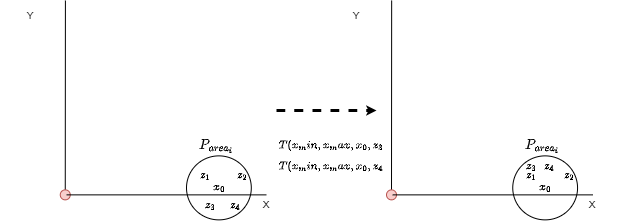
\includegraphics[width=0.8\textwidth]{Method/images/truncation-rq1.png}
  \label{fig:truncation}
  \centering
  \caption{Representation of the remapping algorithm for clustering for points $z_3$ and $z_4$ }
\end{figure}

%\subsubsection{Probability metric $K(x)(Z)$}
%\todo[inline]{Explain the probability metric $K$ we used}

%\newpage
\subsubsection{Algorithm}
The full algorithm for the perturbation:
\begin{algorithm}[H]
  \caption{Full algorithm for perturbing cluster data based on planar/2D-Laplace \citep{DBLP:journals/corr/abs-1212-1984}}\label{alg:rq1}
  \begin{algorithmic}
    \Require $x \in X$  \Comment 2D array of points
    \Require $l \in R^ +$
    \Ensure $z \in Z$ \Comment 2D array of perturbed points
    \State $r = \frac{\sigma}{2}$ \Comment formula 4.1
    \State $\epsilon = \frac{l}{r}$ \Comment Calculating privacy budget \citep{DBLP:journals/corr/abs-1212-1984}
    \State $x_{min} \gets min(X)$
    \State $x_{max} \gets max(X)$
    \State $Z \gets []$
    \For{$point_i \in X$}
    \State $\theta \gets [0, \pi2]$       \Comment Random noise for $\theta$
    \State $p \gets [0, 1]$
    \State $z_i \gets C{_\epsilon}{^{-1}}(p)$       \Comment formula 3.2
    \State $z_i \gets T(x_{min}, x_{max}, point_i, z_i)$ \Comment algorithm 1.
    \State $x_{perturbed} \gets point_{i_x} + (z_{i_x} * \cos(\theta)) $ \Comment add noise to x-coordinate
    \State $y_{perturbed} \gets point_{i_y} + (z_{i_y} * \sin(\theta)) $ \Comment add noise to y-coordinate
    \State append $x_{perturbed}, y_{perturbed}$ to Z
    \EndFor
    \State \Return Z
  \end{algorithmic}
\end{algorithm}
%% We apply the theory for planar laplace proposed by \citep{DBLP:journals/corr/abs-1212-1984}

\subsection{Research question 2}
\todo[inline]{Starts after RQ1}
\subsection{Research question 3}
\todo[inline]{Starts after RQ2}
